\section{Introduction}

Pipelined execution of operators in a query plan is ubiquitous in database management systems~\cite{quickstep-system, monetdb, hyper, vectorwise, elastic-pipelining}. 
A key aspect of pipelining that is exploited by many systems is the prevention of materialization of intermediate results of an operator.  
In a disk-based system, read and write operations involving disk are expensive.
Thus pipelining significantly improves query performance in disk-based systems. 
In the in-memory setting, query processing involves little or no disk involvement. 
Thus data movement across memory hierarchies (e.g. caches to memory) is no longer a bottleneck in query execution.
There is no single aspect that affects the performance of a query, but a combination of factors that jointly impact a query's performance. 

In this work, we revisit the notion of pipelining in the in-memory settings, and present an in-depth study on the effect of pipelined and non-pipelined execution on the performance of a query. 
Our focus is on systems that use block-based style for query processing.
Block-based query processing is used in many systems including single node systems like \sys{}, MonetDB~\cite{monetdb} and Hyrise~\cite{hyrise-website}, Massively Parallel Processing-based systems such as Hive~\cite{hive} and Impala~\cite{impala} which use the Hadoop block abstraction, and key value stores like RocksDB~\cite{rocksdb}.

We first describe the basics of pipelining in query processing. 
In a query execution, data are often streamed between two or more physical relational operators. 
One of the operators in the pipeline acts as a producer operator, that processes the data and streams it to the consumer operator for further processing. 
When the consumer can start processing its input data, even before the producer has processed all of its input, we say that the in the query plan, these relational operators form a pipeline.
A commonly found pipeline found in query plans is made up of selection operator and probe (join) operator, for systems using hash-based join implementations.

We compare the importance of pipelining in query processing in the disk setting and in-memory setting through a hypothetical query example below.

\begin{example}\label{ex:disk}
Let us consider a query which has 1 million intermediate tuples.
We assume that in a disk-based system that uses pipelining, the query runs for 10 minutes. 
Without pipelining, all tuples need to be stored to the disk and brought back.
We assume the latency of a disk read and write to be 1 millisecond.
The time to write the tuples to disk and reading them back to memory is 1 million $\times$ 1 millisecond = 1000 seconds.
\end{example}

Note that in Example~\ref{ex:disk}, the overhead of materializing the intermediate tuples to disk and reading them back is almost twice the query execution time itself. 
Thus there is a big incentive to pipeline the intermediate data, in order to improve query performance. 
Let us consider the same query for in-memory systems.

\begin{example}\label{ex:in-mem}
Consider the earlier query in the in-memory settings by assuming the run time of the query to be 10 seconds. 
We assume the combined read and write latency from cache to memory to be 10 nanoseconds.
Without pipelining, the overhead of writing and reading intermediate data is 1 million $\times$ 10 nanoseconds = 10 milliseconds.
\end{example}

The materialization overhead which was nearly 2x in the disk setting, is merely 0.1\% in the in-memory setting.

Admittedly our example is simple and glosses over many important details. 
However it raises an important question: Is pipelining for in-memory setting as important as the disk setting? 
Answering this question turns out to be challenging, primarily because a combination of factors jointly impacts the performance of a query when there is no I/O bottleneck. 
We first identify these factors, which are parallelism, block size, storage format, sequence of pipelines in a query plan, and hardware characteristics.
The collective space of combinations of these dimensions is large. 
Through our study, we explore this space by identifying the impact of these dimensions on the relative performance of pipelining and non-pipelining strategies.

Prior work has looked at individual dimensions and studied their impact on overall query execution. (Related work is in Section~\ref{sec:pipe-background}).
However to the best of our knowledge, this is the first work aimed at finding the difference between pipelining and non-pipelining strategies, while also studying the impact of various dimensions on this comparison. 
%
%\begin{figure}[t]
%	\centering 
%	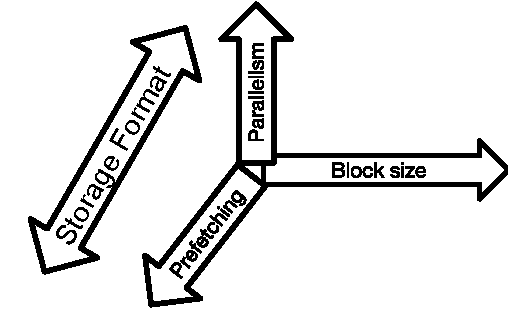
\includegraphics{figures/Dimensions-pipelining}
%	\caption{\textbf{Dimensions that affect the relative performance of pipelining and non-pipelining strategies of query execution}}
%	\label{fig:dimensions-analysis}
%\end{figure}

There are multiple dimensions associated with pipelining in the in-memory settings.
We give a brief overview of these dimensions next, a more elaborate discussion is present in Section~\ref{sec:dimensions}.
\paragraph*{\textbf{Cache behavior}} 
Pipelining and non-pipelining strategies differ based on the \textit{hotness} of input data for the consumer operator. 
In the disk (in-memory) setting, the hotness of the data refers to the data being present in the memory (caches) when the consumer operator starts processing it.

\paragraph*{{\bf Block size}}
Block size refers to the unit of storage for the data movement in query execution. 
A small block size results in a more frequent pipelining and vice-versa.

\paragraph*{\textbf{Storage Format}}
The storage format of stored tables play an important role in query performance. 
We look at how pipelining performance is impacted by the choice of the storage format of the base tables. % row store and column store.

%\paragraph*{\bf{Intermediate output materialization}}: Materialization is not required within a pipeline, which provides two benefits: first, the time to write the temporary output is saved.
%Second, if the temporary output is large, pipelining lowers the memory overhead of the query processing. 

\paragraph*{\textbf{Pipeline Sequence}}
A query plan often has multiple pipelines connected to each other, such that there can be several permutations of these pipelines for execution; each with potentially different performance characteristics. 

\paragraph*{\bf{Parallelism}} 
This dimension is applicable to in-memory based systems with intra-parallel query execution.
Pipelining and non-pipelining strategies result in a different behavior for the extent of parallelism for operators in the pipeline.

\paragraph*{\textbf{Hardware Characteristics}}
Modern database systems try to leverage features provided by the hardware.
We look at one such feature which is prefetching and study its impact on pipelining.

Studying these factors in a single systems requires implementation of pipelining and non-pipelining styles of query processing in the same system.
Systems often have a fixed way of coordinating work execution in a pipeline, which makes the comparison a challenging task. 

Our study is done in a system called \sys{}~\cite{quickstep-system} (system background presented in Section~\ref{sec:sys-background}).
A key aspect that enables us to perform this comparison is \sys{}'s novel scheduler design (described in detail in earlier works~\cite{quickstep-system, DBLP:conf/bigdata/DeshmukhMP17}).
The scheduler relies on a \wo{} abstraction for representing work to be done in a query.
The \wo{} abstraction gives the \sys{} scheduler a powerful control over query execution.
We leverage a key insight that pipelining and non-pipelining strategies result in different schedules of work.
Thus by changing the scheduling strategy, query execution in \sys{} can be done in pipelined or non-pipelined way. 

We compare the performance of pipelining execution strategy to a non-pipelining execution strategy through various combination of knobs. % from Figure~\ref{fig:dimensions-analysis}.
The pipelining and non-pipelining strategies differ in terms of the \textit{eagerness} with which the output of producer is processed by the consumer.
Our analysis uses queries from the TPC-H benchmark~\cite{tpc-h}. 
%We describe our detailed experimental setup in Section~\ref{sec:experiments}.
Although our analysis is based on TPC-H query plans generated by \sys{}, we believe that our methodology should be broadly applicable to other systems.

\paragraph*{\bf{Summary of results and contributions}}:
Our results show that the performance gap between pipelining and non-pipelining strategies is not significant.
This result raises a question that given the high importance of pipelining in the disk settings, why does it not have a significant impact in the in-memory setting?
We present two conclusions based on our observations.

Our first conclusion is that the impact of pipelining on queries depends on the structure of the query plan. 
Queries sometimes contain certain \textit{dominant operators} which take up majority of the query execution time.
The position of such dominant operators in query plan (and pipelines) holds key to the impact of pipelining on the query performance. 
In some queries dominant operator is positioned at the beginning of a pipeline (e.g. selection on \textit{lineitem} table, which is the largest table in TPC-H).
Pipelining typically improves performance of the downstream operators in a pipeline.
Therefore in the presence of a dominant operator the benefits due to pipelining are not significant. 

Our second conclusion is based on an analytical model that compares the performance of queries with and without pipelining in the in-memory environment. 
We consider parameters such as instruction cache misses, data cache misses, number of threads, and block size.
Our model indicates two aspects: First, the gap between these two strategies is not very high. 
Second, as the block size increases, many secondary effects (such as cost of context switching in pipelining) start to diminish.
Micro-benchmarking as well as empirical evaluation on TPC-H query evaluation on \sys{} confirm our findings. 
We summarize our contributions as follows:
\begin{itemize}
	\item We show that the performance of pipelining in the in-memory environments for systems using block-based query processing depends on many dimensions like parallelism, block size, storage format and hardware characteristics like prefetching. 
	\item The benefits of pipelining on query performance cannot be considered in isolation, rather they depend a lot on the query structure.
	\item As block sizes increase, pipelining and non-pipelining strategies start to behave similarly. This is a surprising result given the amount of attention pipelined query processing has received in the past. 
	\item We propose an anlytical model to compare the differences between pipelining and non-pipelining strategies.
\end{itemize}
Our paper is organized as follows: In Section~\ref{sec:pipe-background} we provide a background about pipelining in database systems and also discuss related work.
We give a brief overview of \sys{} in Section~\ref{sec:sys-background}.
We discuss the dimensions associated with this study in Section~\ref{sec:dimensions}.
We present an analytical model to understand the behavior of pipelining and non-pipelining strategies along with micro-benchmarking results in Section~\ref{sec:model}.
In Section~\ref{sec:experiments}, we present the experimental evaluations.
Section~\ref{sec:experiment-summary} summarizes our experimental findings.
Finally, we discuss the future work and conclude in Section~\ref{sec:conclusions}.